\documentclass[11pt]{ieeeconf}
\usepackage{graphicx}
\usepackage{float}
\usepackage{lettrine}
\usepackage{caption}
\usepackage{url}


\newcommand\blfootnote[1]{%
  \begingroup
  \renewcommand\thefootnote{}\footnote{#1}%
  \addtocounter{footnote}{-1}%
  \endgroup
}

\title{Bumper Car Sumo}
\author{Jaden Simon - simonjaden223@gmail.com \\ \and
	   Melvin Bosnjak - meco0597@gmail.com \\ \and
	   Daniel Humeniuk - d.humeniuk@utah.edu \\ \and
	   http://bumpercarsumo.weebly.com/}

	   
\begin{document}

\maketitle

\begin{abstract}
Americans are not having fun anymore. The weight of capitalism is forcing families to work 60-hour weeks for low pay, leading to decreased enjoyment and productivity. An affordable and efficient form of entertainment would help solve this issue. In order to promote this, our group is designing a bumper car battle royale game. The project will have intuitive controls, simple yet fun mechanics, and a robust interface to allow for easy development. Continued play testing during development will allow us to monitor these objectives. Our ultimate goal is mutual enjoyment between us and our players.
\end{abstract}

\section{Introduction}
Entertainment is a fundamental part of the human experience. While some lucky few are able to derive satisfaction from their career, most people need something else to entertain themselves. This is the focus of our team's project: to develop an entertaining game with widespread appeal.

 The most important criteria of our game’s success are cost and entertainment efficiency. Our game must yield high levels of fun per minute played, while keeping costs as low as possible without compromising the entertainment value. Competition in games is a key element for high entertainment value \cite{vord:03}.  Because of this, our team decided to create a game where player-controlled robots attempt to push each other out of an arena. To facilitate gameplay, our robots need to be easily pushed around by other robots. Controls should be easy to enhance playability, though not too easy. We need a way to detect game conditions, such as when a robot is out of bounds or when a player wins. This could be done with a human referee, but that would take away immersion of the game. Because some players may not have friends to play with, it is desirable to have an AI to play against. 

Since cost is a contributing factor to our design, we will want to use existing technologies as much as possible. Robots can be constructed as a two-wheeled platform with wireless modules, similar to a Segway. They will be controlled through a web interface accessible by a wide variety of devices. Computer vision libraries will allow us to track the location of each robot if painted differently. Exact positioning solves the problem of detecting game conditions, plus giving us plenty of information to use for a basic AI. 

Our goal, above all else, is that our game is fun. Playtesting will be a major component of our design process, rethinking aspects of the game if it is not fun. Costs will be mitigated, but entertainment value will never be sacrificed for savings. Player enjoyment is our primary measure of success.

% Olliie bot figure
\begin{figure}[H]
\centering
\captionsetup{justification=centering}
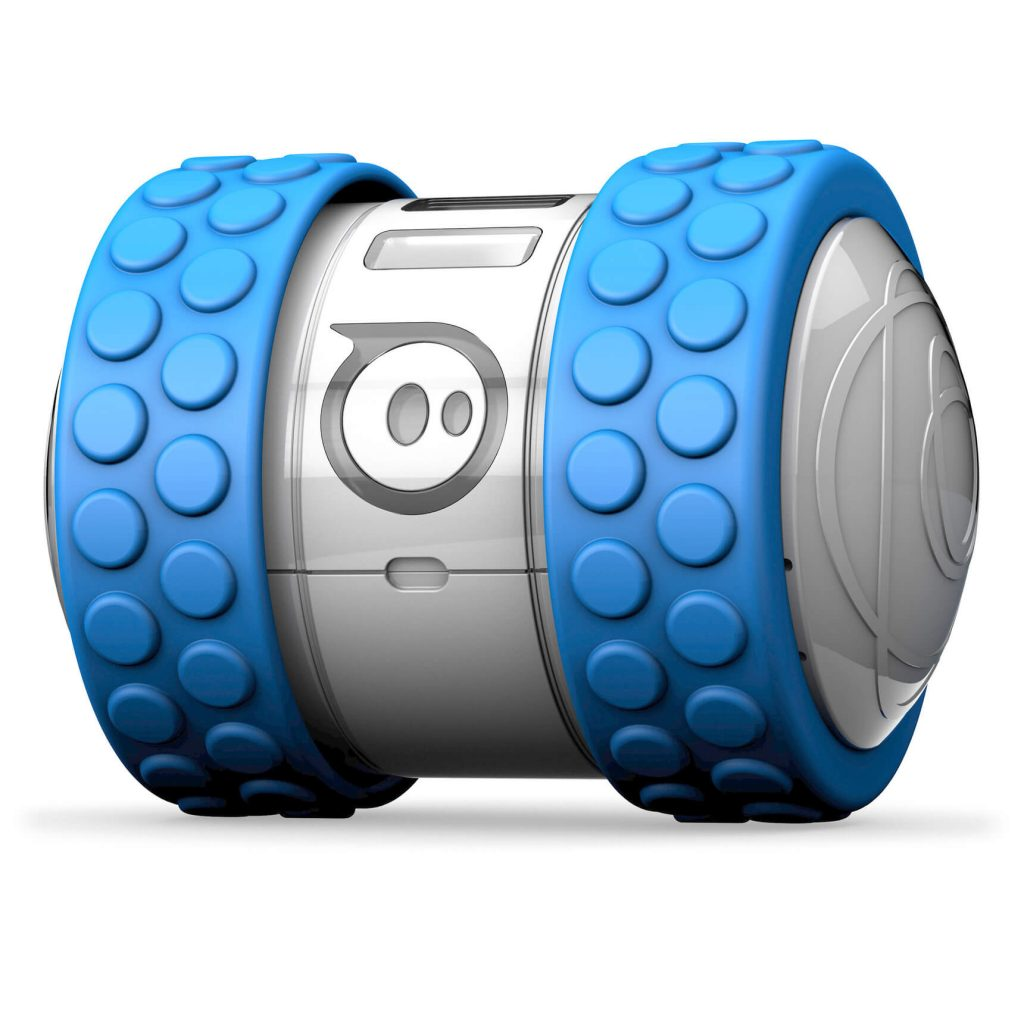
\includegraphics[width=0.5\textwidth]{images/SumoBot.png}
\caption{The Ollie from Sphero\\Source: Adapted from \cite{ollie:19}}
\label{Ollie}
\end{figure}

\section{Background}
The biggest component to our project is the robot. Two-wheeled wireless robots already exist and are mass produced, such as the Ollie (Fig \ref{Ollie}). While the Ollie has many of the features we require for our project, it does not give the level of control necessary to make our game a reality. On top of that, it is expensive at over \$80.00 per unit. The specifications for the Ollie are freely available online and will help guide us through the design of our own robots.


Tracking the robots would be a huge undertaking, but luckily there exists an open-source computer vision library called OpenCV. OpenCV provides algorithms to scan an image and identify desired patterns \cite{opencv:19}. With this, tracking can be done with only a camera, a computer, and a small bit of code. 

\section{Design}

To complete the project, we will need a main control mechanism (a hub), robots, controllers, and tracking. A centralized hub will be the core of the project, which will coordinate the other three components. The robots will use a custom PCB with an inertial measurement unit (IMU) and low-voltage motor driver, able to communicate via WiFi through an ESP8266. Our controllers will have both a physical and software interface. An overhead camera will be used to monitor the locations of our robots, which will be combined with IMU data for an extremely accurate positioning system. Separating these four components allows for simultaneous development by our team members.

\subsection{Hub}
The hub will be a Raspberry Pi device that will have a few functions:
It will capture the game state from a camera peripheral. The camera will be hooked directly into the Raspberry Pi and the hub software will have to continuously take the frame data from the camera and pass it as an input to openCV. The hub software will then associate the color of the robot with the location openCV outputs to keep track of each robots location. This process will be on its own thread that will have to share memory with the thread that is running the game loop. This allows the game logic to know the location of robots at all times. This means we will have to eliminate race conditions with thread locks. A flowchart is shown in \ref{flowchart}.

Another thread will be hosting a server. The server will have communication with the controllers, and each robot. This thread will be a loop that takes in player inputs, updates the game state, then sends the appropriate commands to the robots. The hub will most likely have to hold many game models to support the game modes.

Fig. \ref{flowchart} shows the basic illustration of the game. If time allows, then our AI implementation will be done on the hub. This component of the project requires no custom hardware and can be done entirely in software. The Core hub software will take at most a month for full development and testing. 

% Game design figure
 \begin{figure*}[!t]
  \centering
  \captionsetup{justification=centering}
      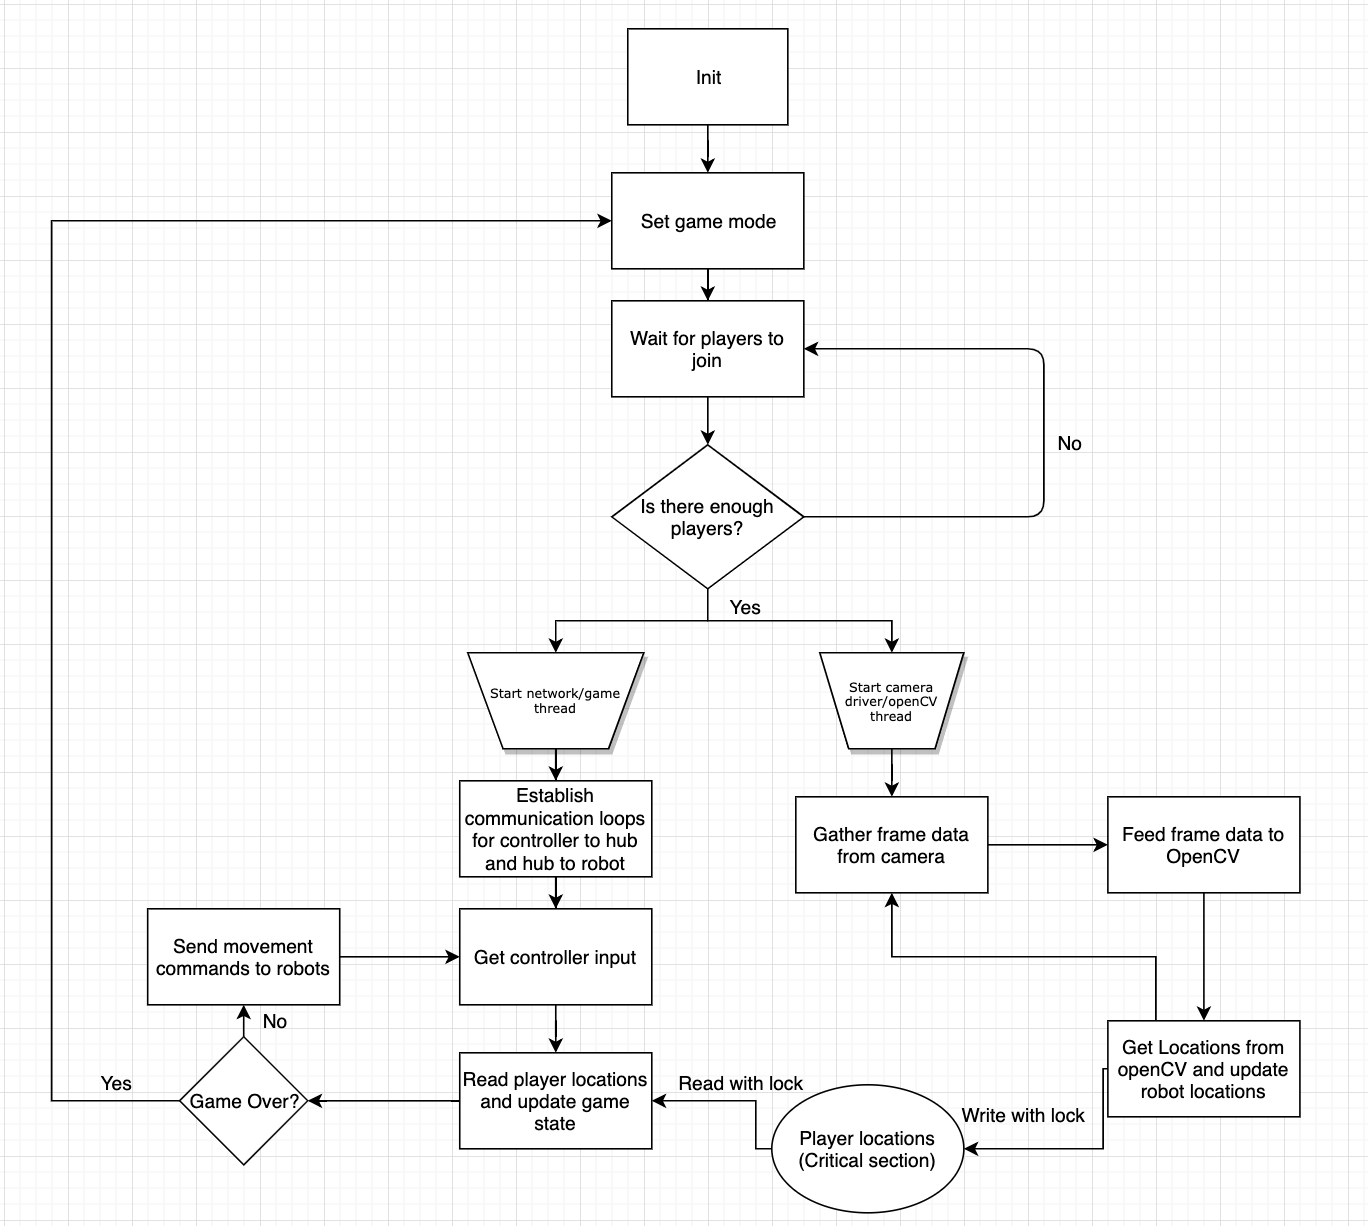
\includegraphics[width=14cm]{images/Flowchart.png}
        \caption{Overall game design}
        \label{flowchart}
\end{figure*}

% Maybe split each component into new sections (Robot Design, Hub Design, Controller Desgin)
% That way they can each have their own subsections
\subsection{Robot}
% More pictures
Our robots will be cylindrically shaped with two wheels on each side of the body that can move in either direction independently (Fig. 3). In order to move forward, both of the wheels will spin at the same time at the same rate. To move backwards, the same principle applies in the opposite direction. Rotating the robot left or right requires spinning the motors in opposite directions. Because of space and cost limitations, we are aiming to keep our robots small with a maximum length of 6 inches and maximum height of 3 inches. Ideally, the robots will weigh between 8 and 16 oz, lightweight enough for quick acceleration yet hefty enough to push each other around. Designing the robot can be subdivided into 5 components: custom PCB, power subsystems, powertrain, shell, and software.

% Robot design figure
 \begin{figure}[H]
  \centering
      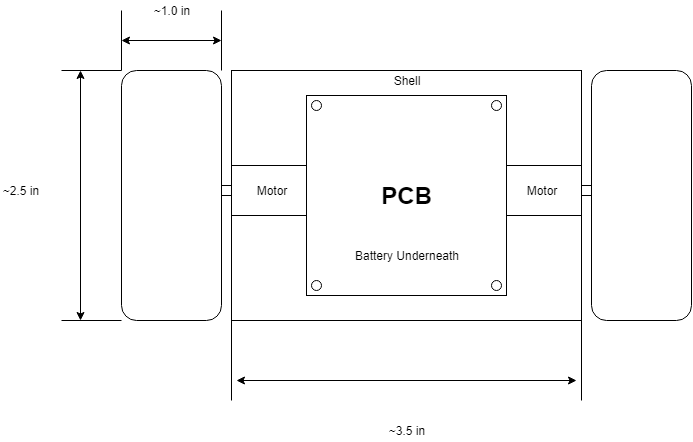
\includegraphics[width=0.5\textwidth]{images/RobotSchematic}
        \caption{Basic robot layout}
        \label{RobotFig}
\end{figure}

A custom PCB with an ESP-12S will be the heart of our robots, driving our motors as well as providing voltage regulation and wireless communication. Additionally, an inertial measurement unit (IMU) will be used for positioning data. This data will be relayed back to the hub for additional processing. Programming an ESP-12S requires a USB-to-UART chip and a USB connector. These components are very common and will not be a major factor in our design. A low-voltage motor driver is required due to the fact that our highest voltage available is only 3.7V. Currently, the PCB is designed to be 2x2 inches, giving plenty of room inside the shell for the battery, motors, and gears.

To reduce system complexity, we are using a single 3.7 lithium polymer battery to power the robot. The ESP-12S requires 3.3V which means we need a voltage regulator to convert the variable battery voltage to a steady 3.3V. A battery charging IC on the board lets us charge our batteries without having to disassemble the robot. Most charging ICs can safely provide 500mA, charging in a reasonable time. Our custom board will average around 120 mA during normal operation, though the motors can consume up to 2A combined at max load, depending on the motor. Because the motors require large amounts of current, they will need to be powered directly by the battery rather than the on-board voltage regulator. With a 2000 mAh battery we can expect 2 hours of playtime, taking 4 hours to charge at 500mA. The ESP-12S chip has a peak current draw of 500 mA, so we should plan on using a voltage regulator that can support at least 600 mA.

We want our motors to provide enough force to push other robots around. With a little bit of physics we can estimate the force required to begin pushing a robot. Assuming our robots weigh 1 lb, our wheels are rubber, and the arena is made of wood, we would require around 2 newtons of force to overcome static friction. We will account for a margin of error with the friction coefficient as well as the friction from the pushing robot to give us a design requirement of 3 newtons. Since we have two wheels, each wheel will need to provide 1.5 newtons of force. Our wheel diameter is planned to be around 1 cm in diameter, giving a goal torque of 0.75 N-cm or around 76 g-cm. Motor specifications will often list their stall torque, however, this stall torque is not sustainable for long periods of time. To give an additional margin of error, we will have a desired stall torque of 5 times our goal torque, or 375 g-cm. Considering the huge variety of DC motors available, some additional research will have to be done to find the right motor. We will likely have to use a gear ratio between 10 and 20 to achieve the desired torque using standard DC toy motors. The gears will be 3D printed along with the shell. It is important to note that using gears to increase torque will decrease how fast the wheels spin proportionally. Starting from a motor running at 10000 RPM and using a gear ratio of 20, we get a final wheel RPM of 500. A RPM of 500 with 2.5 inch wheels travels at about 4 MPH, which is plenty fast for our little robots.

Finally, our robots will be contained in neat little shells. Each shell should be a different color so that our OpenCV code can easily track them. PLA+ seems like a good choice for 3D printing material, being cheap yet strong enough to sustain some hits. Many of the specifics of the shell have yet to be determined since they are dependent on the physical dimensions of our components. However, we do know that the shell will be designed with a top and bottom half, with screw holes to allow for easy assembly and disassembly. Some sort of internal mounting platform would be needed to secure the PCB. A USB-port should be accessible outside the shell so that we can reprogram and charge our robots without disassembly. 

The software running on the robot will be extremely simple, interpreting commands from the hub to drive the motors and send back IMU data. Some additional code could be written to monitor battery charge or change how much power is delivered to the motors. Considering all these details, the robot will take up to 3 months to fully develop and test due to its requirement of custom hardware, though a significant amount of work has already been done.

\subsection{Controller}
% Talk about using Wii balance board and/or game console controller 
% Maybe talk about other ways to control the robots ? 
The controller provides the opportunity to add interesting game mechanisms that are unique to our game. We have been discussing ideas for unique control options and have come up with several ideas. We are developing and interfacing multiple controllers to give players a choice in their play style as well as providing backup plans if one or more turn out to be unenjoyable. The ideas we are pursuing are utilizing a web server, Wii Balance Board, and Nintendo controllers. The web server involves players logging into a website and using keyboard inputs to move the robots as they watch the game through the web camera. The Wii Balance board, as seen in Fig \ref{Wii}, allows for a more interesting and challenging style of play by utilizing player movement. The Nintendo controllers will include Super Nintendo and Nintendo 64 controllers that will plug directly into the Raspberry Pi Hub. Each controller will be discussed in further detail below with their respective priority level.

% Wii fit board figure
\begin{figure}[h]
\centering
\captionsetup{justification=centering}
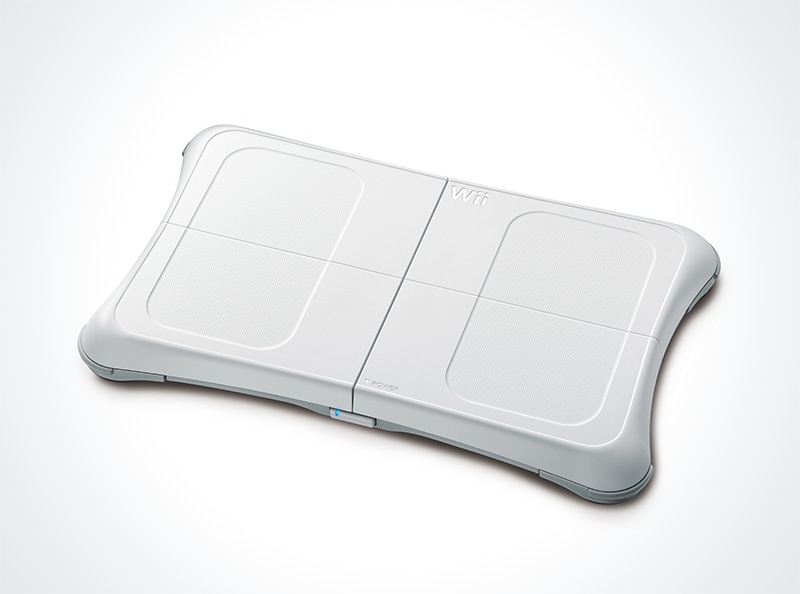
\includegraphics[width=0.45\textwidth]{images/wii.png}
\caption{The Wii Balance Board is an ideal candidate for a unique control system\\ Source: Adapted from \cite{wiiboard:19}}
\label{Wii}
\end{figure}

A web-based control system is currently the cheapest controller option with some possibilities to enhance the playing experience. The users will need to use their personal WiFi enabled laptops to log into a website we will develop for the game and select a robot to play as. The website will be streaming a live feed of the game play area via the web camera that will also be handling the tracking capabilities. The players will receive a brief overview of the controls that are enabled on their keyboards and are then allowed to select the robot of their choice. Once a robot is selected, any physical controller in the game area will be disabled. The robots will be driven forward, back, left, and right with the use of key presses. The key presses will be sent to the Hub which will process the information and pass it on to the respective robot. We will work on limiting latency between button presses and movement of the robot. This controller will be medium priority as the implementation will be more of a challenge than the Wii Fit Board but it is simple enough to not require a large allocation of our time.

If time allows, we will make further use of OpenCV and add extra features to the web interface. The robots will be tracked on screen with and player names will be displayed above their respective robot. This also adds potential to enhance the game with power-ups for certain game modes. We will also enhance the controller by adding graphics and notifications when games are won, lost, begin, and end. The added features will add to the appeal to this controller.

The Wii Balance Board promises an interesting controller experience. We will interface with the board to receive output from standard user inputs to the board. From there, we can interpret the data in the control hub. There are many references online that will assist in interfacing with the controller. The Wii Balance Board uses a Bluetooth profile called Human Interface Device Profile which we will need to interface with and interpret the data as we need. As seen in \cite{homebrew}, the Wii Balance Board uses 16-bit pressure sensors. With four sensors total, it will be possible to enable two sensors to assist in driving one motor. Once the device has been interfaced with, we will collect input from the device by standing on it and leaning forward, back, left, and right. Once we can see what the average output will be for these measurements, we can effectively write the software for the Hub to interpret the data to drive the robot. The board feature will provide users with both interesting and challenging gameplay. This controller requires the highest priority as it will take time to ensure we are interfacing properly with the board's Bluetooth profile. 

There are many variations of Nintendo controllers currently available online that will be the fastest controller option to implement. The authors of \cite{controller:19} inform us that no additional drivers are needed for many of the available controllers which will ease the process of interfacing them with the Hub. Fig \ref{Controllers} shows a Super Nintendo controller on the right and a Nintendo 64 controller on the left. The Super Nintendo controller has a simple D-pad to steer the robots which will makes the directional input easier to interpret and the extra buttons will be used for speed control. The Nintendo 64 controller has a D-pad for steering as well as a joystick. We can use the joystick to control the speed and direction of the robot. The Hub will account for both types of steering depending on which controller is being used. This controller remains at the lowest priority as the interfacing has already been done. The biggest task with these controllers is to interpret their output data and relay the result to the robots.

% USB controllers
\begin{figure}[H]
\centering
\captionsetup{justification=centering}
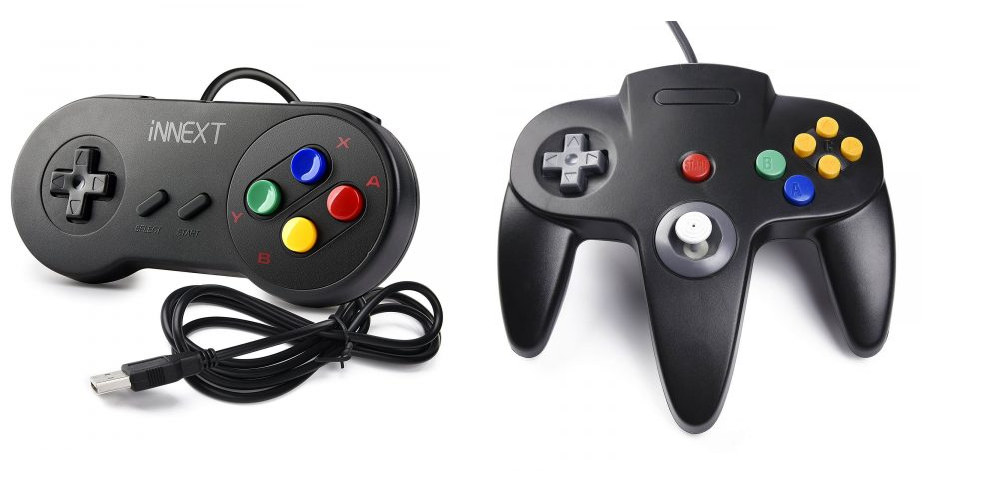
\includegraphics[width=0.5\textwidth]{images/controllers.png}
\caption{Two USB controllers to be used \\ Source: Adapted from \cite{controller:19}}
\label{Controllers}
\end{figure}

While electing to use Nintendo controllers is not the most original option, this is the option that we are the most confident in as a backup plan. The USB allows for a fast and painless implementation. There is also benefits to the players having familiarity with game paddles which will allow them to enjoy the ease in controlling the robots. We can also add interesting ideas during the play-testing phase of the project. Once all required components of the game are complete, features will be added that utilize the extra buttons on the Nintendo controllers. With the Nintendo controllers, we are safe to explore other controller options such as the web server and Wii Fit Board and know that the Nintendo controllers will be an viable fallback. 

The choice to implement multiple controllers provide more options for the players and gives us more possibilities to explore our creativity. This also gives room for us to continue adding controllers that can be implemented with extra game modes offered, similar to the business model of Downloadable Content (DLC) that is featured in most modern video games. The controllers have been selected to provide the users with a new and challenging experience and will be modified and added to until they provide that experience. 

\subsection{Tracking}

Tracking will be done by the hub using a camera and OpenCV. The casings for each robot will be designed in such a way to allow for easy identification by algorithms. Players who leave the camera's field of view will be considered eliminated by the hub, preventing control of the robot by the player. Since our camera will be static, the total play area is limited by our camera's height and field of view. Our play surface will be monochromatic which increases our tracking capability, though we should be able to track with an arbitrary surface. The timeline for tracking is largely dependent on the hub and the robot, though 2 weeks seems like a reasonable amount of time.

\subsection{Arena}

The arena for the game will be a flat piece of circular wood, similar to a tabletop without legs. The diameter will be 6ft and no more than an inch off of the ground. There will be four pillars attached at equal parts from one another around the circumference of the arena which will extend upwards. The pillars will extend upwards form a cone shape and meet in the middle. The point of intersection will support the Hub and the camera. 

Some game modes will require a bumper to be added to the edges to ensure all the objects within the arena stay within the arena. The bumpers will be four inches wide and sit an inch above the main game area. For the Wheel-Ball game mode (see section Game Mechanics for more detail on this game mode), the bumpers will not cover two small openings on opposing sides of the arena. This opening will allow a ball to enter and a team to score. The bumpers will be created using simple wood pieces that will be connected together and wrap around the parameter. 

Our ideal arena will be dynamic in nature but this will be added during the polishing stages of the project and if time allows. We will make the arena dynamic by cutting holes in the board and saving the cutout pieces. By using actuators, we will drive the cutout pieces up and down on the board to add obstacles. For the Wheel-Ball game mode, we will cut out two holes on either end of the board and drive the actuators down to enable an opening large enough for the ball to enter. Once the ball enters the cutout area, the detection software will notify the Hub of a score. The actuator will drive cutout piece up and release the ball back into play. This will create a more even flow to the gameplay. A dynamic game arena will add a lot of interesting play options and require players to utilize more skill and tact in game.

The dynamic game arena will contain the ability to control the bumpers along the parameter. The actuators under the arena will drive the bumpers up or down depending on the game mode. This takes the responsibility from the players to ensure the game will operate properly and allow the Hub to handle these features automatically. This also adds the possibility to catch robots after they fall off the board during the Battle Royale mode. This will be implemented by the tracking system. Once the robot is out of bounds, the Hub will halt the robot and it will remain out of bounds on the bumper. When the game resets, the bumpers will raise and the Hub will guide the robots back into place. The dynamic game arena has the potential to create a smoother game play experience for the users and eliminating the need to reset the game manually. 

\section{Game Mechanics}

%Let's call the rocket league game play mode Wheel-Ball. Kinda like football but for a robot with a wheel instead of a foot
There will be many game modes to select from. The primarily plan was to design the game arena to accommodate only one game mode. The team has elected to enable for multiple game modes to provide longevity to the product. Each game mode will require the players to change their play styles and tactics from game to game. When a game finishes, the results are displayed, and the players have the option to replay the match, change controllers, or select a different game mode.

\subsection{Battle Royale}

The first game mode that the group proposed is Battle Royale. The players will drive their robots into other robots in attempts to knock them out of the game arena. The tracking software will monitor where the robots are on the board and detect when a robot goes out of bounds and shut it off. The last robot on the board will win. If there is a circumstance when the remaining robots exit the board at the same time, the winner will be determined by the detection software and it's interpretation of which robot exited first.  

\subsection{Team Battle Royale}

Team Battle Royale game mode contains many of the same rules as the previous Battle Royale with the exception that players will be working together in teams against other teams. This game mode requires a lot of play testing to determine what additional features the Hub will require. To eliminate stalemates and standoffs, the Hub will reserve the ability to temporarily retake control from the players and separate them if the robots remain in the same area for a specified length of time. A stalemate will be defined as two or more robots attempting to push one another with no avail. The motor drivers will relay heat sensor information and notify the Hub that they are exerting power with no movement from the motors. The Hub will take over if this event occurs to ensure that power in the robots is conserved as well as protecting the motors within the robots. The players will have the option of selecting two teams with two to four players per team or four teams with two players per team. Because of the physical nature of the game, friendly fire is a possibility and the Hub will take note of the times players take out their own team members. The game ends when all but one team is remaining on the game arena. 

\subsection{Wheel-ball}

Wheel-ball is another team based game mode. The teams will work together to move a ball across the arena and into the opposing team's goal. It is up to the teams on how they wish to accomplish this goal and it is possible that one player acts as a goalie. There are some more rules required for this game mode as it will be possible for a robot to completely cover their team's goal line. This requires more interactions from the Hub but it is necessary to enable a fair game will be played. Each time the ball enters into a team's goal, the opposing team is awarded a point, even if a team scored on itself. The time limit for the games will be five minutes. Once the five minutes has expired, the team with the most points wins the match.

To ensure the players are playing by the rules, the Hub and detection software will work together to ensure the players are behaving. If a player attempts to block their own goal zone, the Hub will take temporary control of the robot, move it away from the goal, and deactivate it for ten seconds. The diameter of this zone will be painted on the game arena with a color that the detection software will be able to detect. The rule will be considered violated if 30\% or more of the robot is within this zone for over three seconds. This will allow for players to think about their decisions and how to defend their goal without getting too close. 

\subsection{Smash-n-Bash}

The Smash-n-Bash game mode will be implemented if enough time permits. This game mode will assign each player a health bar that will detriment each time the player is hit by an opponent. To accomplish this, the video detection software will track the directions the players are heading in to determine if the player was hit or doing the hitting. With each hit detected, the hitting player will accumulate points. Once a player's health is depleted, the Hub will take control of the robot and move the robot off screen. For cases with head-on collisions of the robots, the video detection software will add points to both players as well as take away health from both players. The player with the most points will be declared winner. The game mode will provide a challenging experience for the players as the players will have to dodge and outmaneuver their opponents. 

\section{Timeline}
In order to finish our project before demo day, we have created a timeline as seen in Fig \ref{schedule}. While the deadlines listed here are not set in stone, it should give us a good idea of what we need done by when. The length of the bars represent about how long it should take to complete the task. Each group member is assigned to a certain task dependent on the bar's color, though there is some flexibility there as well. Some of the tasks are dependent on the completion of previous tasks, so it is important for us not to get too far behind schedule.

% Graphic of timeline
 \begin{figure*}[!t]
  \centering
  \captionsetup{justification=centering}
      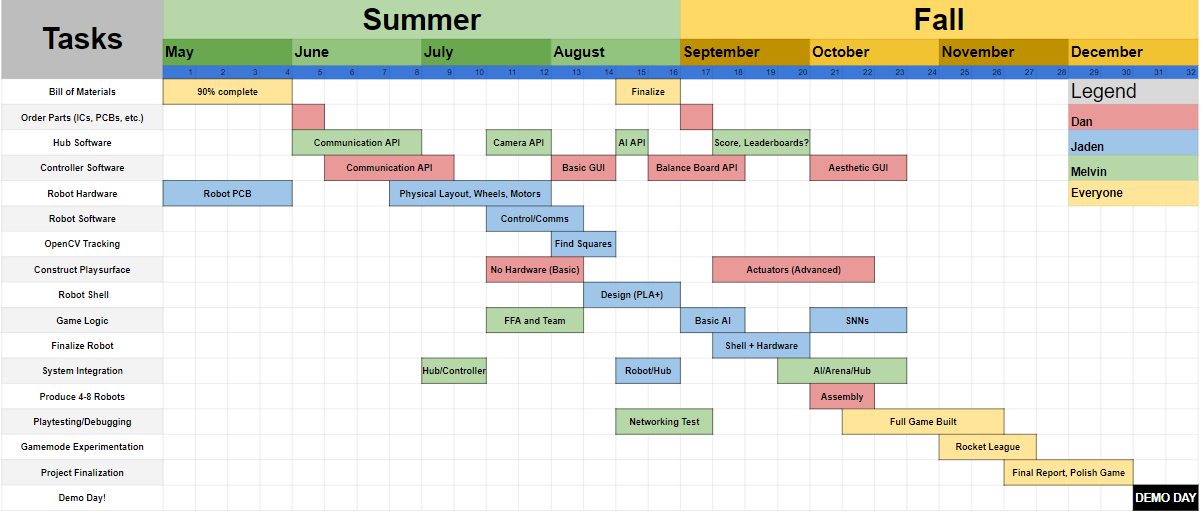
\includegraphics[width=\textwidth]{images/schedule.png}
        \caption{An itemized schedule for the group}
        \label{schedule}
\end{figure*}

\subsection{Spring}
For the remaining month of May we will finalize our required parts list. This includes verifying we have the correct parts, checking availability, and price calculations. 

\subsection{Summer}
The summer will consist of ordering and gathering the resources needed as well as detailed design for each component of the project. Basic documentation of our hardware and software interfaces will be completed by the end of the summer. We will complete a basic software interface and start experimenting with hardware interfaces. If time allows then we can create a basic play surface, since it is not dependent on the completion of any singular component.

\subsection{Fall}
Most of the legwork for the project will be done during the fall. With all components gathered and the design completed all that will be left to do is to assemble, test, and finalize documentation. Each project component will be worked on simultaneously. Integration between the four components of the project will not take long if our interfaces were designed correctly, perhaps only a week or two. The minimum requirements of the project is planned to be completed and tested a month before the demo day. A large amount of extra time allows us to experiment with additional features that will hopefully add to the entertainment value.

\subsection{Component Assignments}
As already discussed, the project is separated into 4 key components. Each component will have a single group member act as lead developer. Robots and tracking will be managed by Jaden. Development of the hub and its communication protocol will be done by Melvin. Dan is tasked with creating the software controller interface as well as working on variations of hardware interfaces. Fig \ref{schedule} provides a graphical representation of the separate responsibilities of each component. The integration of our multiple components will begin in the middle of the fall. The next section will detail the milestones each member must accomplish in order for the project to succeed on schedule.

\section{Milestones}
% Every person needs at least 5 milestones 
Each group member will have at least 5 milestones to their assigned component: 

\subsection{Melvin}
For Melvin, his component will be heavily involved with the Hub device, so the first milestone will be getting a basic network connection with multiple ESP8266 client devices. This will be done over the summer. This should be quick as we have demonstrated working a client server network connection for the prototype. During Demo day this will be shown with the ability to control each robot wirelessly as this will require handling multiple wireless connections simultaneously.

The second milestone will be creating a communication API with the Hub. This will consist of designing a protocol to support controller to hub commands and hub to client commands. This will be tested once we test connecting the whole system together. This will also be shown with the ability to control each robot wirelessly. This will also be done this summer.

The third milestone will be to interface the hub device with the camera peripheral that we will use to capture the game state. This will include ordering the appropriate camera for our tasks, figuring out how to gather frame data from the camera, and propagating that frame data to OpenCV. This will be shown by the ability to detect when a robot has gone out of the play area. This will be done later in the summer.

The fourth milestone will be to create a model that captures and processes the game state within the hub so that it can easily control game mechanics. This will have to continuously read the game state from the camera API and store it in its internal model. Based on the model, it will then send the appropriate commands/data to clients. This will be made very modular in order to support multiple game modes. This will be done in the fall along with the last milestone. This will be shown by the hubs ability to manage a game and keep track of score, winner etc.

The last milestone will be to integrate and test the hub with the whole system. This will depend on the state of each other component, but we would like to leave at least a month before demo day to complete this milestone in order to leave time for integrating stretch goals and finalizing the project. This will be shown by the system working as expected.

\subsection{Jaden}
Jaden will be working on the design of the robot which includes the tracking software on the hub. His first milestone is the completion of the robot prototype PCB, showing all components are functional. This first demonstration includes programming the ESP-12S, controlling a motor, charging a battery, and using the IMU. Completing the robot PCB allows the other members to start interfacing with it, so it is important to get it done as soon as possible. The next milestone is developing the software on the robot, allowing the hub to communicate with it wirelessly. Sending commands from the hub to the robot PCB to control a motor will demonstrate that this was completed. The next goal for the robot design is creating the shell and gears necessary to complete the robot. Completion of this milestone will be shown by fitting the PCB, battery, motors, and gears within the shell. The robot's USB port should also be accessible. For the last robot design milestone, Jaden will demonstrate that the entire robot works as a cohesive unit. That is, the robot can be programmed and controlled by the hub wirelessly, driving around on battery power alone.

The final two milestones for Jaden involve tracking and AI. Tracking of the robots will be implemented with OpenCV and provide the hub software with location data. If the arena and hub are complete, then this can be demonstrated by having the hub output current player locations while moving a robot around the arena. Otherwise, demonstrating the tracking capability will involve detecting colored pieces of paper, representing our robots, moving around in front of a camera. Creating a basic AI using the tracking data will be the final milestone. The AI software should run on the hub, controlling a robot autonomously. A basic AI will simply try to stay within the arena while driving towards other robots. This can be demonstrated by running the AI on one robot, then driving another robot around the arena. If the AI works then it should follow (and hit) the human-controlled robot without exiting the arena.


\subsection{Dan}

Dan is primarily working with the controllers and the handy work for the game arena. The largest and possibly most challenging task he has been charged with is interfacing with the Wii Balance Board which is his first mile stone. This aspect of the game deals with Bluetooth which is unfamiliar to the team as a whole which is why this will be worked on over the summer. Modders in the WiiBrew \cite{homebrew} community have been working with the device and there are several resources which will lighten the load with this task. This will also require a lot of data collection to determine what outputs are given for different movements and how they could be best interfaced with the Hub. The completion of this milestone will enable the group to progress in the Hub software and other aspects of the project.

The next milestone for Dan will be the completion of the game arena. This will not require any hardware or software but a working play area must be made for testing of the movement of the robots and the tracking via the web camera. This milestone will be completed before the end of the summer as well so the group can begin integrating other aspects to be completed over the summer. The early development of the game arena will also allow for any improvements to be made to the aesthetic, design, and appearance can be done with plenty of time before the presentation day.

The first milestone to be completed during the fall will be the development of the graphical user interface for the web server. The interface will be conceptualized with the use of sketches and approved by the team. The completion of this interface will provide the group with a controller that will connect with the Hub and testing can begin to determine if there any latency issues and other bugs that may occur. This milestone will be completed by the end of August.  

The next milestone for Dan is creating Wii Balance Board API. This will be accomplished in September or earlier if possible. The API will insure that the Hub will be able to interpret the data from the Wii Balance Board. The summer will allow for ample time for Dan to test the balance board for different inputs and be able to determine what kinds of data will be output by the device. This is a critical step as playtesting the robots with the balance board will be required to ensure that no latency issues will occur as well as the output of the board being properly interpreted by the Hub. The successful completion of this milestone by the end of September will allow for additional features to be added during the later months of the project.  

Dan will be charged with interfacing the Nintendo controllers with the Hub in October. This will require some additional software components as the controllers contain multiple ways to control the robots. The milestone should not require too much attention as the controllers are compatible with the Raspberry Pi so no extra effort is needed with creating an API. The output will need to be interpreted properly by the Hub which can be tested as the robots will be completed at this point in time. The milestone will ensure that the users will have multiple controller options to chose from and additional features can be added to enhance the gamplay provided by the controllers.

The last milestone for Dan is implementing the actuators onto the game arena to enable dynamic gameplay. This milestone is optional as the other components of the game take priority over this feature. This milestone will be completed in November and a new game arena will be purchased and made to accomplish this task. It is imperative that the existing game arena remains as is to ensure that there is a functioning game arena for the demonstration day. The completion of this milestone will require an additional micro-controller to receive communication from the Hub to drive the actuators up and down. This milestone will add a layer of polish to the game and game modes.

\section{Resources}
% Flesh out this section (full BOM) 
% Part number, lead time, unit cost, quantity, form factor, etc.
\subsection{Bill of Materials}

Each robot will require 2 DC motors with wheels, several batteries, a PCB that includes an ESP8266 microcontroller and motor drivers for each DC motor, and a casing to enclose and protect the internals. The casing will be designed and 3D printed by our group. Various ICs and small electrical components will be required based off our circuit designs. The design, testing, and implementation of the robot will take the bulk of the time required for this project. Many of the parts for the robot have been determined, though we have not narrowed down which vendor we will use for each component (Fig. \ref{robobom}). Please see our website for the most recent version of the BOM including the datasheets for each component.

% Robot BOM
 \begin{figure*}[h]
  \centering
  \captionsetup{justification=centering}
      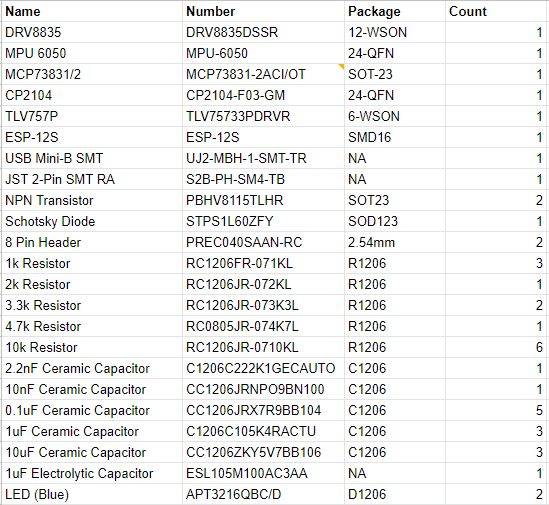
\includegraphics[width=0.75\textwidth]{images/bom.png}
        \caption{Current BOM for our robot}
        \label{robobom}
\end{figure*}

A Raspberry Pi will act as the hub, handling all game mechanics and user-robot interactions. The Raspberry Pi 3 Model B+ has a quad core 1.4GHz processor which should be enough processing power for these tasks. Tracking is a fundamental component of the hub and will require a camera, ideally with high resolution and FPS. The options for the camera are the Raspberry Pi camera and the Logitech C922x Pro Stream Webcam. Software on the hub will depend on multiple open source libraries to function, though will still require significant custom software to operate.

The playing field will be constructed out of a simple table top with some 2 x 4's to hoist up the camera, with power and data cables running down to connect to the hub.

\subsection{Vendor List}
% List all vendors with contact information 

\section{Group Logistics}
In order to stay on top of our set deadlines, our group will be meeting at least once a week to discuss current tasks, issues we have experienced, and new ideas for our game. These meetings are logged on our website. Because Melvin will be in Idaho for the duration of the summer, our meetings will have to be digital and infrequent. In the fall we will resume the weekly meetings.

The individual milestones presented in the Milestones section will keep the members on track and clear defined goals. Our milestones will allow us develop components separately and work together during the integration. 

\section{Risk Management}
% Describe risks for each task, some might not have any

For the Hub device, some potential risks with this is latency, and computing power. The Hub device has many responsibilities such as camera I/O, game logic, handling many network communication channels, and running OpenCV. In order to reduce these risks the Hub will be using UDP connections with each client and multi-threading each task. This will also be done over the summer. This will require a device that has multiple cores, wifi capabilities, and a fast processor. That is why we chose the Raspberry Pi 3 Model B+.

Perhaps the biggest risk with the robot design is the development of the PCB. Getting a new PCB can take a couple of weeks, not including the time to solder the components. Debugging PCBs thus have a very high latency; you will not see if your fix actually worked for at least a week, if not more. For comparison, in software all you have to do is compile and rerun the code to test it, taking a matter of minutes. That is why we are starting the robot PCB now, before summer even begins. This gives us a huge amount of time to debug the board. We will also be triple-checking our PCBs before they get sent off for fabrication. Some of the PCB design is based off already functioning products (ref. \cite{feather}), which should increase the likelihood that it works the first time. The parts we are using are fairly common and cheap, especially if we order from China. Ordering internationally has the unfortunate side-effect of taking upwards of two months to arrive. We have tried to mitigate the possibility of not getting all of our parts on time by ordering them at the start of summer. That way if we realize we need different parts or the parts arrived broken, we have enough time to order more. As a final resort, we can always order parts from reputable domestic companies at significantly higher cost.

The biggest risk potential noted with our controllers is the Wii Balance Board. The potential risks include challenges interfacing with the board as well as its viability as a fun controller option. The interfacing risk is already mitigated by utilizing the resources provided by a strong hobbyist community that specializes in interfacing with Nintendo Wii products \cite{homebrew}. There is the potential risk that the data we get from the board will be difficult to interpret and use. This risk will be mitigated by testing multiple methods such as leaning movements or applying pressure with heel and toe presses. We have also considered that the controller may be frustrating to use. This risk can be eliminated by reverting to the other controller options we have included. The risks for the Wii Balance Board are successfully be eliminated by testing multiple controlling methods, utilizing existing open source projects, and having backup controllers if it turns out to cause frustration over enjoyment.

The other controller that contains potential risks is the web server interface. The implementation of this controller system is straight forward but communicating from a server to the Hub may adds to the noise of the constant WiFi communication already at play. We have discussed adding more ESP8622s to connect with the Hub. There are many other solutions that will need to be explored if the added WiFi creates enough noise to cause other parts of the game to malfunction.  

The USB Nintendo controllers do not pose any risks to the project. If the risks from the Wii Balance Board and the web server interface prove to be too great, we will use the Nintendo controllers in their place.  

The game arena does pose potential risks but they do not effect the project. The standard game arena does not pose any risks as the construction of the board will be straight forward and not include any complicated features. The dynamic game arena does pose risks but this is a feature that will only be implemented if time permits. The standard board will suffice for demonstration if the dynamic game arena cannot be completed in time.

\section{Testing}
Much of our time spent testing will be focused on robot design and user experience. The most complicated part of our robot will be the integration of a battery, but once that is complete we will focus on debugging software communication protocols. In addition, play-testing of the project is fundamental to our success. We must ensure that our game is entertaining through repeated testing of robot collisions and the user interface. Collisions with robots should feel powerful and the user interface should be responsive and free of frustration. Beyond that, we will need to experiment with the durability of our robots to make sure they do not break during play.

\section{Project Demonstration}
% Describe what will be highlighted in the demo 

On demo day, we hope to achieve a minimum requirement of 4 robots, basic user interface, and a single game mode. While 4 robots will provide enough competition to be entertaining, we ideally want 8 robots to allow more people to play. Basic user interface would only have options to control the robots in the 4 cardinal directions. More game modes are simple to implement but add enormous entertainment value.

\subsection{Setup}
First players connect to our web server through a device of their choice. Connections made in previous rounds will be preserved. Players then choose an available robot to play as. Each selected robot must be placed in designated spots, which will have to be done by humans. Once the hub detects that all robots are in the play area, the game can begin. 

\subsection{Game Round}
Each game round will depend on the game mode. In all of our Battle Royale game modes, players are eliminated if their robot leaves the play area. For the free-for-all Battle Royale, the game round ends when all but one player is eliminated. If team mode is implemented, then a game round ends when only a single team remains. The Wheel-ball game will track the scores of each team and utilize a time limit. At the end of the Wheel-ball round, the team with the most points wins.  

\subsection{Post Game}
If we are able to meet our minimum requirements, then additional features will be added to aid user experience. This would include post game reports that contain information about the player such as eliminations, maximum speed, or the biggest hit taken. After any post game reports, our demo will start again at the setup.

The dynamic game arena will assist in post game reset if it can be implemented in time. The Battle Royale game mode will use the automated bumpers and Hub software to ensure that the robots can leave the game arena but not continue past the lowered bumpers. The Wheel-Ball mode will control the actuators under the cutouts to release the balls once a score has been made. By implementing this, the users are not required to pick up the game ball every time a score is made. This feature can only be implemented with time permitting but it will make the game more automated and easy to play a second round. 

\section{Project Status}
% Current status of our project
% Robot PCB pretty much
The current status of our project largely comes from our prototype. We have demonstrated wireless communication in a client server architecture. We have also gotten the first version of our robot PCB fabricated as seen in Fig \ref{prototype}. The PCB was tested and had some problems. The main problem stemmed from an incorrect footprint that shorted a components V\textsubscript{cc} input to ground. The error the mistake created caused the waste of the components that were ordered for the board as well as the PCBs. We have learned from the first version which will make for a much more robust second version.

% Prototype PCB
\begin{figure}[H]
\centering
\captionsetup{justification=centering}
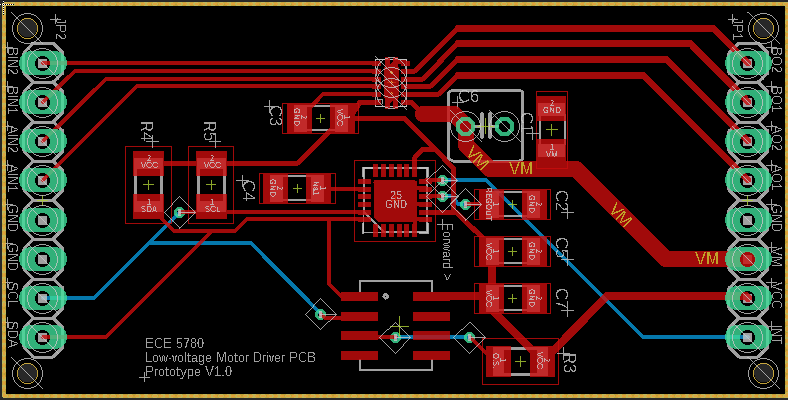
\includegraphics[width=0.5\textwidth]{images/prototype.png}
\caption{The prototype board layout}
\label{prototype}
\end{figure}

Our prototype utilized the gyroscope on the STM32 Discovery Board and two ESP8266 WiFi chips to wirelessly control a motor. The WiFi chip transmitted data via UDP to the other WiFi chip that is connected to a motor driver. The motor driver powered a DC Motor and it will spin clockwise, counterclockwise, or remain still depending on the provided signal. The first attempt at data transmission was using the HTTP protocol but we found that the latency was too high to provide reliable control to the motor. Using the gyroscope also proved to be a successful experiment as we were able to control a single motor with an interesting control mechanism. We also learned of the limitations of a gyroscope. An accelerometer would have been a much more robust tool to determine movement as opposed to the STM's attached gyroscope.  

Considering that the robot will take the bulk of the time on this project, we have already started work on its final PCB. The current design features an ESP-12S as the microcontroller, a DRV8835 to drive the motors, a CP2104 to convert USB signals to UART, a TLV757P LDO voltage regulator, a MCP73831/2 to charge the battery, and a MPU-6050 as the IMU (Fig. \ref{roboboard}). Our USB port is a mini-B since the cables are pretty common and the port is sturdy compared to a micro USB port. The battery is connected through a standard JST PH 2-pin connector rather than just soldering the wires onto the board. This allows us to swap out the battery much more readily. We chose to develop our own board with the ESP-12S embedded rather than purchase an external module because having everything in one system not only looks nicer, but also significantly reduces the final cost.

% Final PCB
\begin{figure}[h]
\centering
\captionsetup{justification=centering}
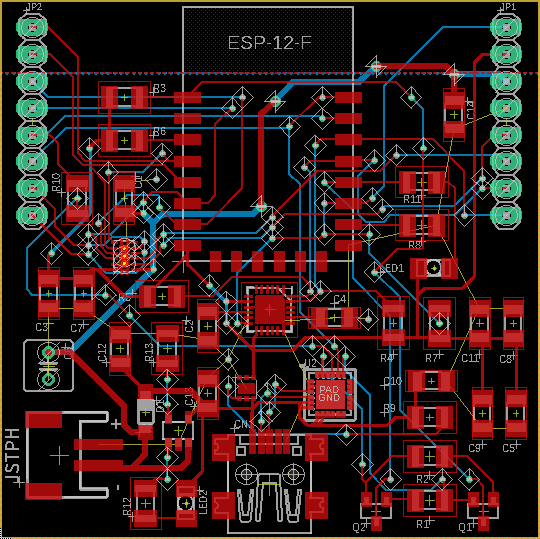
\includegraphics[width=0.5\textwidth]{images/RobotBoard.png}
\caption{The (almost) final robot board}
\label{roboboard}
\end{figure}

\section{Conclusion}
% Summarize entire proposal, include lessons learned so far (management/team/engineering) 
% Include biggest risks, analyze task dependency 
% Final advertisement of project 

\bibliographystyle{IEEEtran}
\bibliography{IEEEabrv,bib/ref}

\end{document}